\documentclass{beamer}

\mode<presentation> {
  \usetheme{CambridgeUS}
  %\setbeamertemplate{footline} % To remove the footer line in all slides uncomment this line
  %\setbeamertemplate{footline}[page number] % To replace the footer line in all slides with a simple slide count uncomment this line
  \setbeamertemplate{navigation symbols}{} % To remove the navigation symbols from the bottom of all slides uncomment this line
}

\usepackage{graphicx}
\usepackage{booktabs}
\usepackage{svg}
\usepackage[]{algorithm2e}
\usepackage[francais]{babel}
\usepackage[utf8]{inputenc}

%----------------------------------------------------------------------------------------
%   TITLE PAGE
%----------------------------------------------------------------------------------------

\title[Challenge Data ENS]{Projet Plume Labs: prédire la qualité de l'air à l'échelle de la rue}

\author{Louis THIRY, Alexandre SAINT-DIZIER}
\institute[MVA]
{ENS-Cachan}
\date{\today}

\begin{document}
\bibliographystyle{unsrt}

\begin{frame}
\titlepage
\end{frame}

%\begin{frame}
%\frametitle{Overview}
%\tableofcontents
%\end{frame}

%----------------------------------------------------------------------------------------
%   PRESENTATION SLIDES
%----------------------------------------------------------------------------------------

\begin{frame}
\frametitle{Choix du projet}
\begin{itemize}
  \item un problème concret et ambitieux
  \item mêle apprentissage et physique
  \item découverte des séries temporelles
\end{itemize}
\end{frame}

\begin{frame}
  \frametitle{Formalisation du problème}
  $\rightarrow$ prédiction de série temporelle entière
  \begin{itemize}
    \item une série temporelle = 1 donnée
    \item 28 variables explicatives (19 statiques, 9 dynamiques)
    \item 17 données d'entrainement (3 par ville)
    \item 12 données de test (2 par ville)
  \end{itemize}
  Peu de données
\end{frame}

\begin{frame}
\frametitle{Remarques sur les données}
\begin{itemize}
  \item Comportement physique des trois polluants très différent.
  	\begin{center}
  		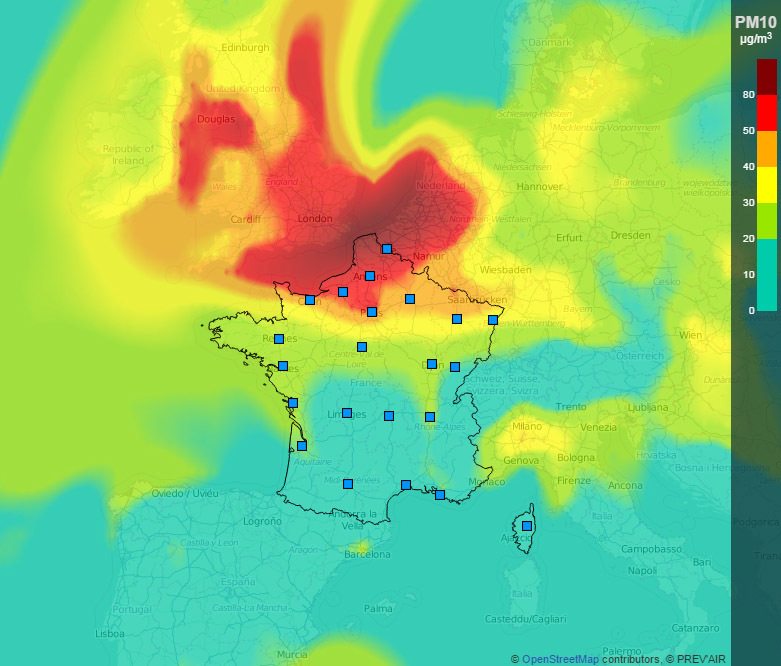
\includegraphics[width = 0.5\linewidth]{images/francepm10.jpg}
  	\end{center}
  \item Données météo identiques par ville
  \item Pas de données géographiques
\end{itemize}
\end{frame}

\begin{frame}
\frametitle{Remarques sur les données}
\begin{itemize}
	\item Pas d'informations précises sur les routes
    \begin{center}
    	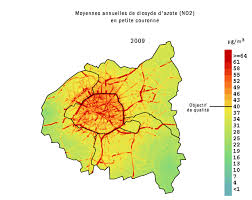
\includegraphics[height=5cm]{images/parisno2.jpg}
    \end{center}
  \item problème de somme de cosinus et sinus
\end{itemize}
\end{frame}

\begin{frame}
  \frametitle{Exploration des données}
\begin{figure}[H]
	\captionsetup{labelformat=empty}
	\minipage{0.33\textwidth}
	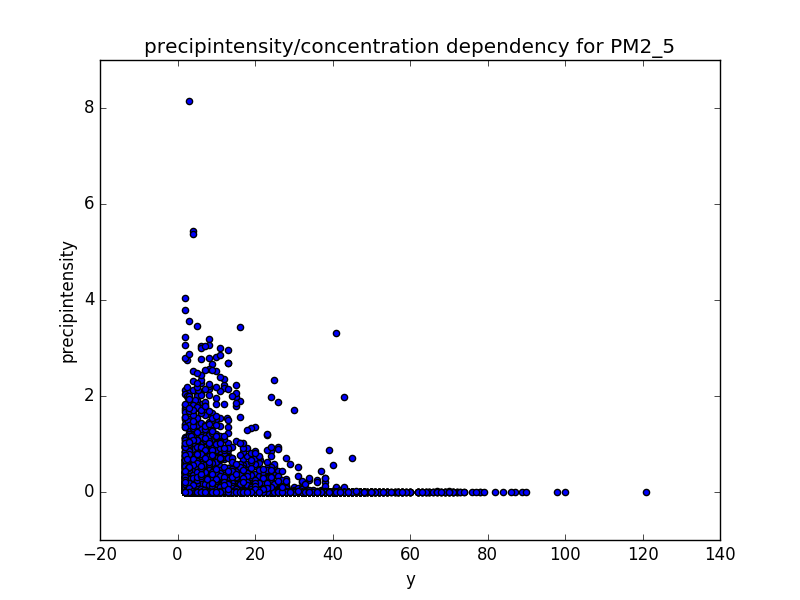
\includegraphics[width=\linewidth]{images/PM2_5_precip_y.png}
  \caption{$PM_{2,5}$/précipitations}
	\endminipage\hfill
	\minipage{0.33\textwidth}
	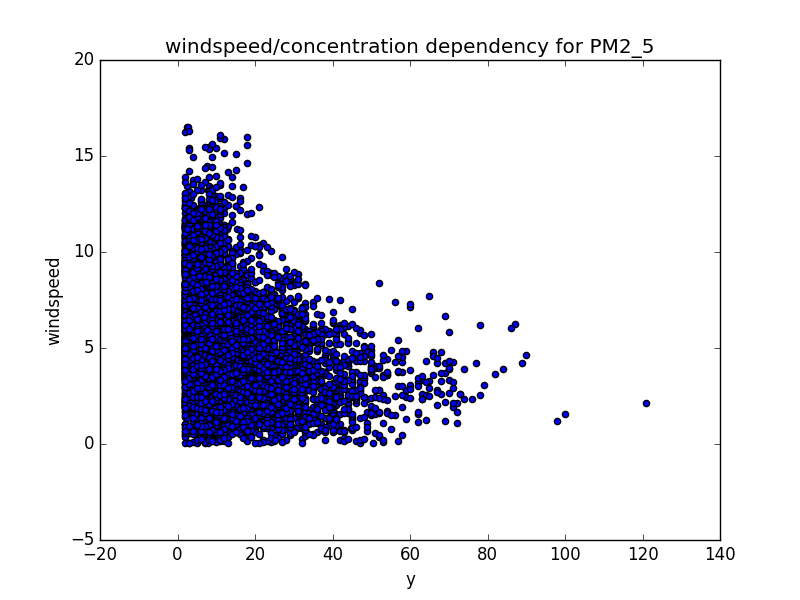
\includegraphics[width=\linewidth]{images/PM2_5_windspeed_y.png}
  \caption{$PM_{2,5}$ /vitesse du vent}
	\endminipage\hfill
	\minipage{0.33\textwidth}
	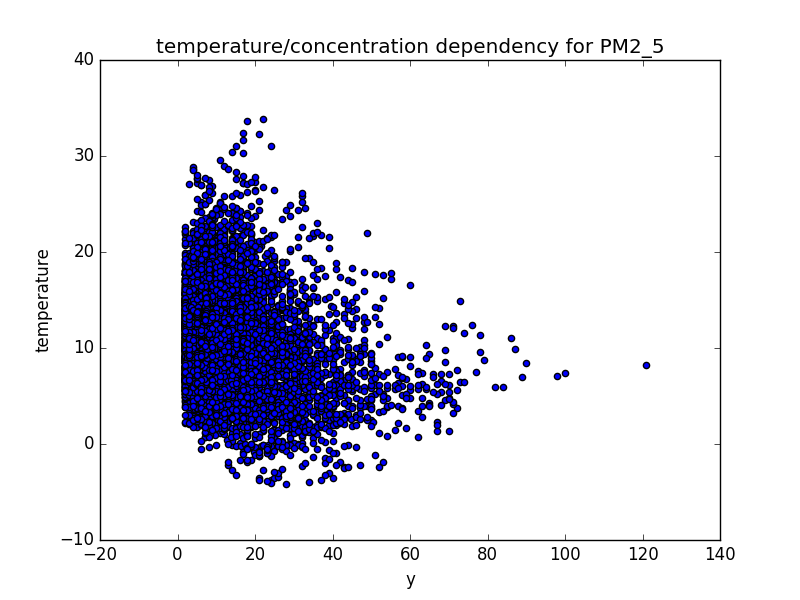
\includegraphics[width=\linewidth]{images/PM2_5_temp_y.png}
  \caption{$PM_{2,5}$ / température}
	\endminipage\hfill
\end{figure}
\end{frame}

\begin{frame}
  \frametitle{Exploration des données}
\begin{figure}[H]
	\captionsetup{labelformat=empty}
	\minipage{0.33\textwidth}
	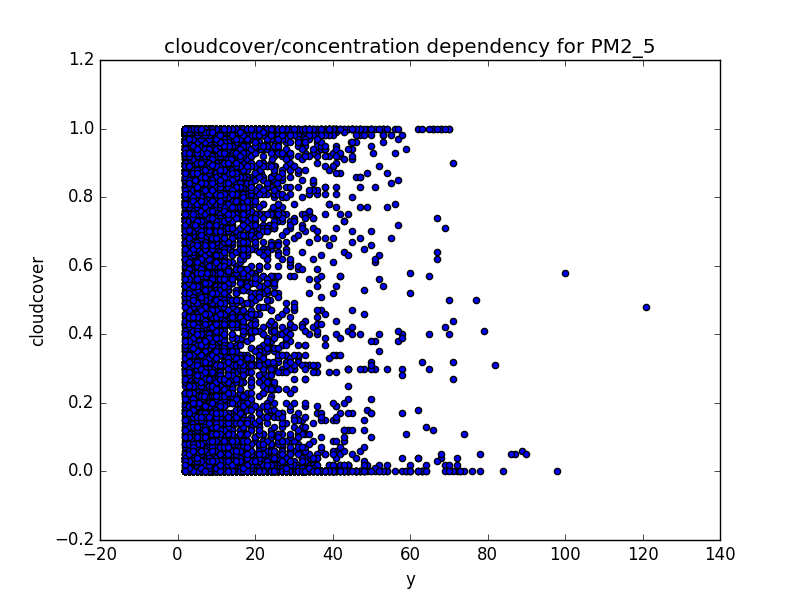
\includegraphics[width=\linewidth]{images/PM2_5_cloud_y.png}
  \caption{$PM_{2,5}$/ennuagement}
	\endminipage\hfill
	\minipage{0.33\textwidth}
	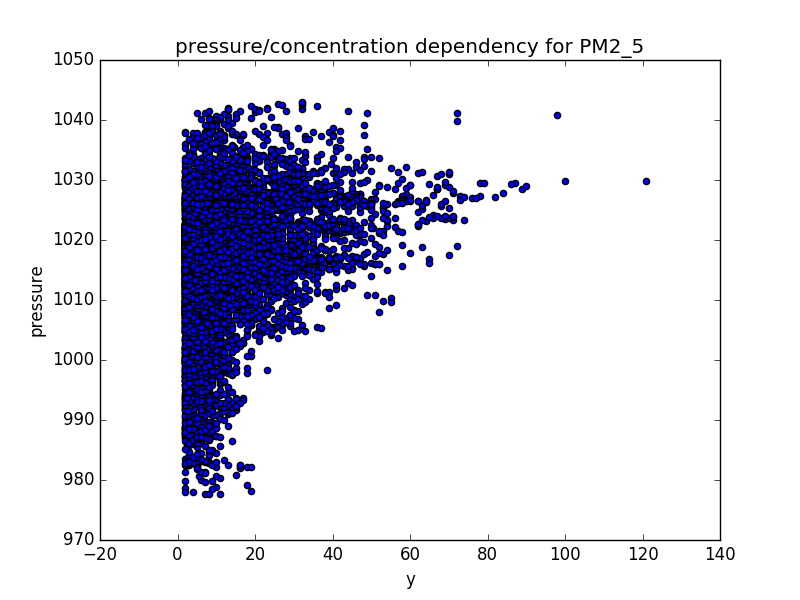
\includegraphics[width=\linewidth]{images/PM2_5_pressure_y.png}
  \caption{$PM_{2,5}$ /pression}
	\endminipage\hfill
	\minipage{0.33\textwidth}
	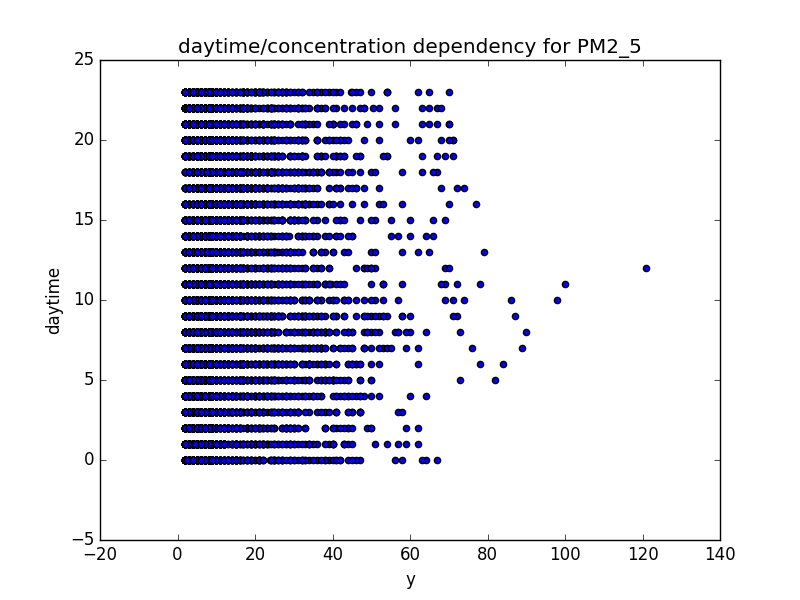
\includegraphics[width=\linewidth]{images/PM2_5_daytime_y.png}
  \caption{$PM_{2,5}$ /heure}
	\endminipage\hfill
\end{figure}
\end{frame}

\begin{frame}
  \frametitle{Exploration des données}
\begin{figure}[H]
	\captionsetup{labelformat=empty}
	\minipage{0.33\textwidth}
	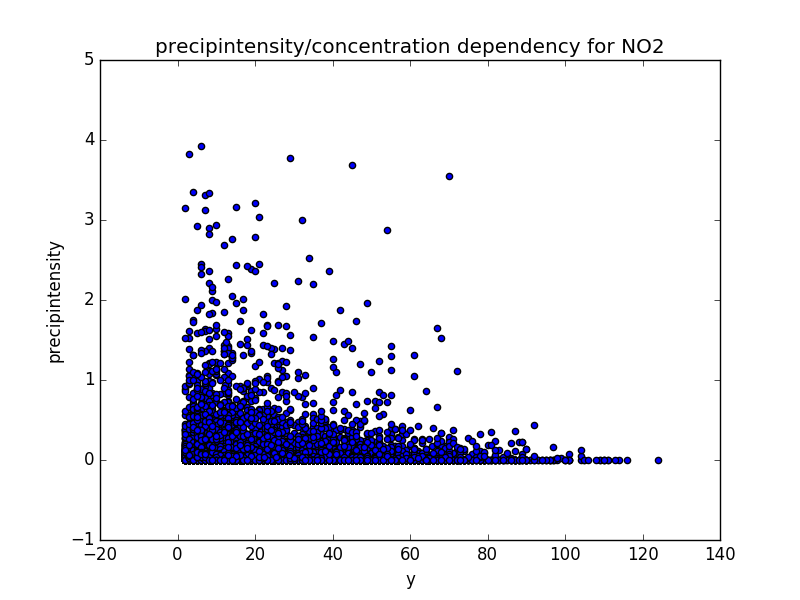
\includegraphics[width=\linewidth]{images/NO2_precip_y.png}
  \caption{$NO_2$/précipitations}
	\endminipage\hfill
	\minipage{0.33\textwidth}
	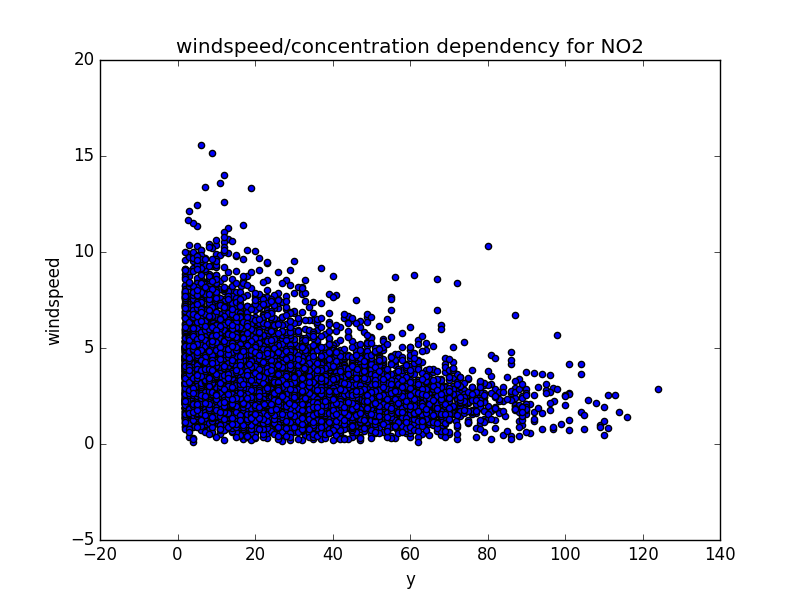
\includegraphics[width=\linewidth]{images/NO2_windspeed_y.png}
  \caption{$NO_2$ /vitesse du vent}
	\endminipage\hfill
	\minipage{0.33\textwidth}
	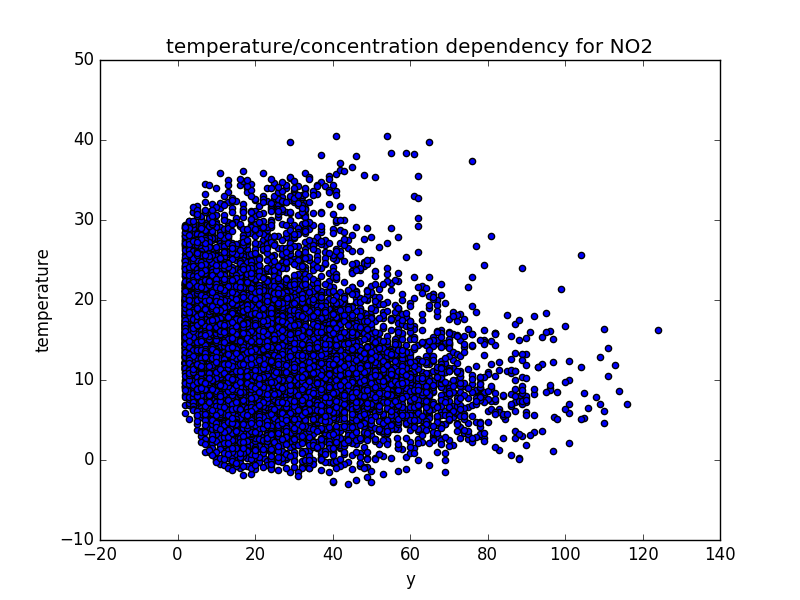
\includegraphics[width=\linewidth]{images/NO2_temp_y.png}
  \caption{$NO_2$ / température}
	\endminipage\hfill
\end{figure}
\end{frame}

\begin{frame}
  \frametitle{Exploration des données}
\begin{figure}[H]
	\captionsetup{labelformat=empty}
	\minipage{0.33\textwidth}
	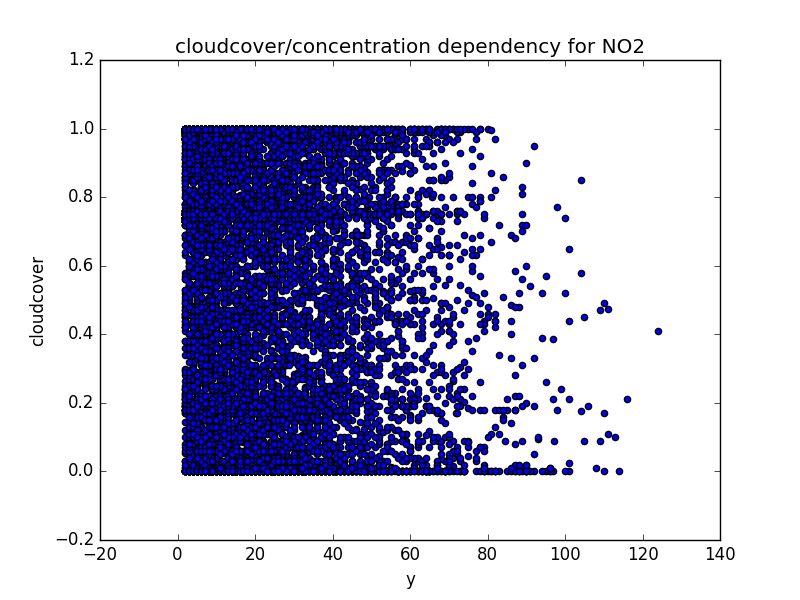
\includegraphics[width=\linewidth]{images/NO2_cloud_y.png}
  \caption{$NO_2$/ennuagement}
	\endminipage\hfill
	\minipage{0.33\textwidth}
	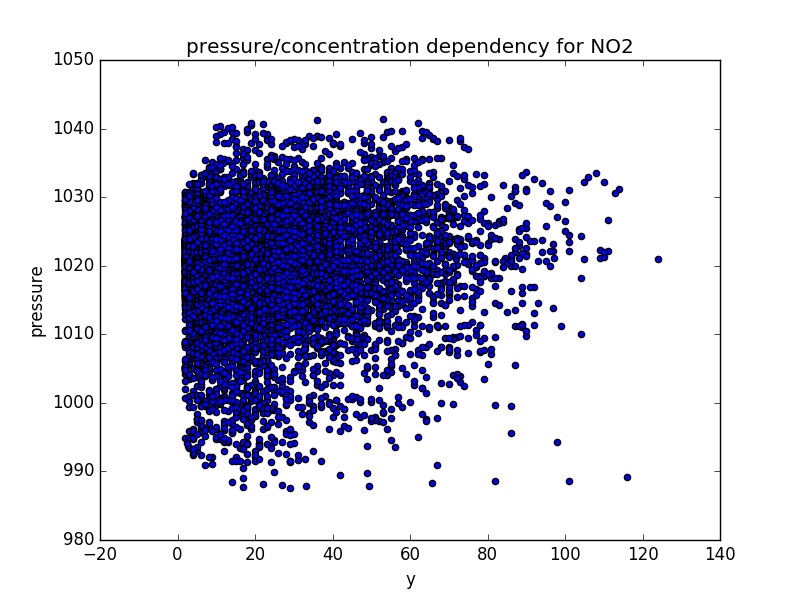
\includegraphics[width=\linewidth]{images/NO2_pressure_y.png}
  \caption{$NO_2$ /pression}
	\endminipage\hfill
	\minipage{0.33\textwidth}
	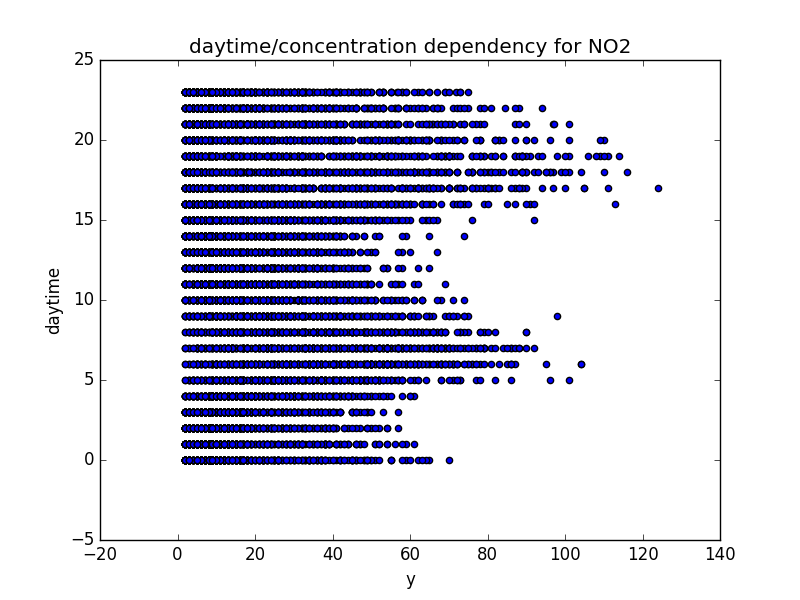
\includegraphics[width=\linewidth]{images/NO2_daytime_y.png}
  \caption{$NO_2$ /heure}
	\endminipage\hfill
\end{figure}
\end{frame}

\begin{frame}
\frametitle{Revue}
\cite{NO2reg}: pollution en $NO_2$ par variables statiques.
\begin{itemize}
  \item 4 types de routes
  \item valeurs du traffic routier
  \item l'altitude est donnée
  \item les batiments sont classés par taille
  \item 24 données d'entrainement pour une seule ville
\end{itemize}
Régression linéaire et à noyau : 60\% de précision.
\begin{center}
  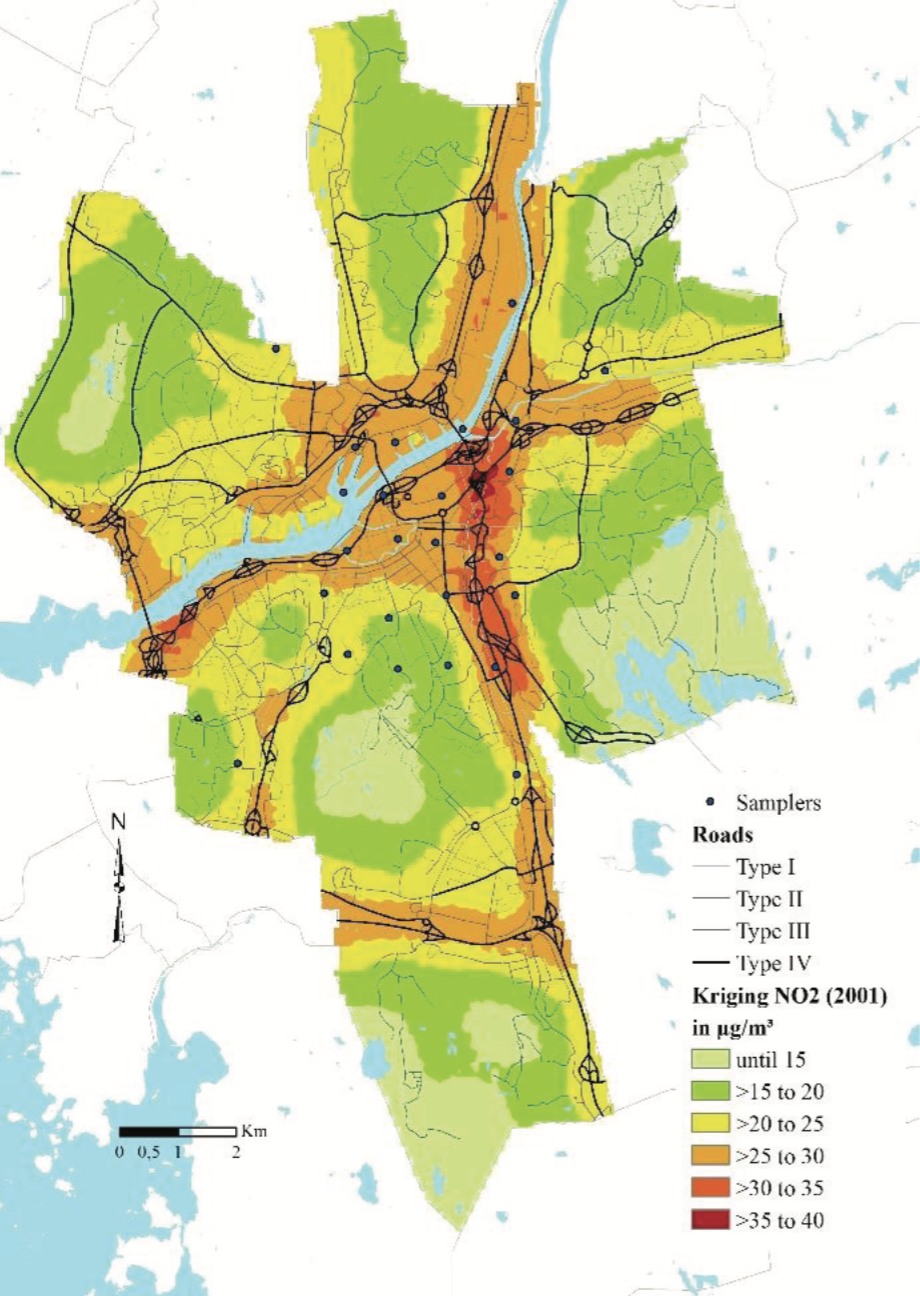
\includegraphics[height=4cm]{images/pollution_gothenburg.png}
\end{center}
\end{frame}

\begin{frame}
\frametitle{Revue}
\cite{PMreg} : pollution en particules ultrafines.
\begin{itemize}
    \item données météorologiques et statiques
    \item capteurs mobiles:
\begin{center}
  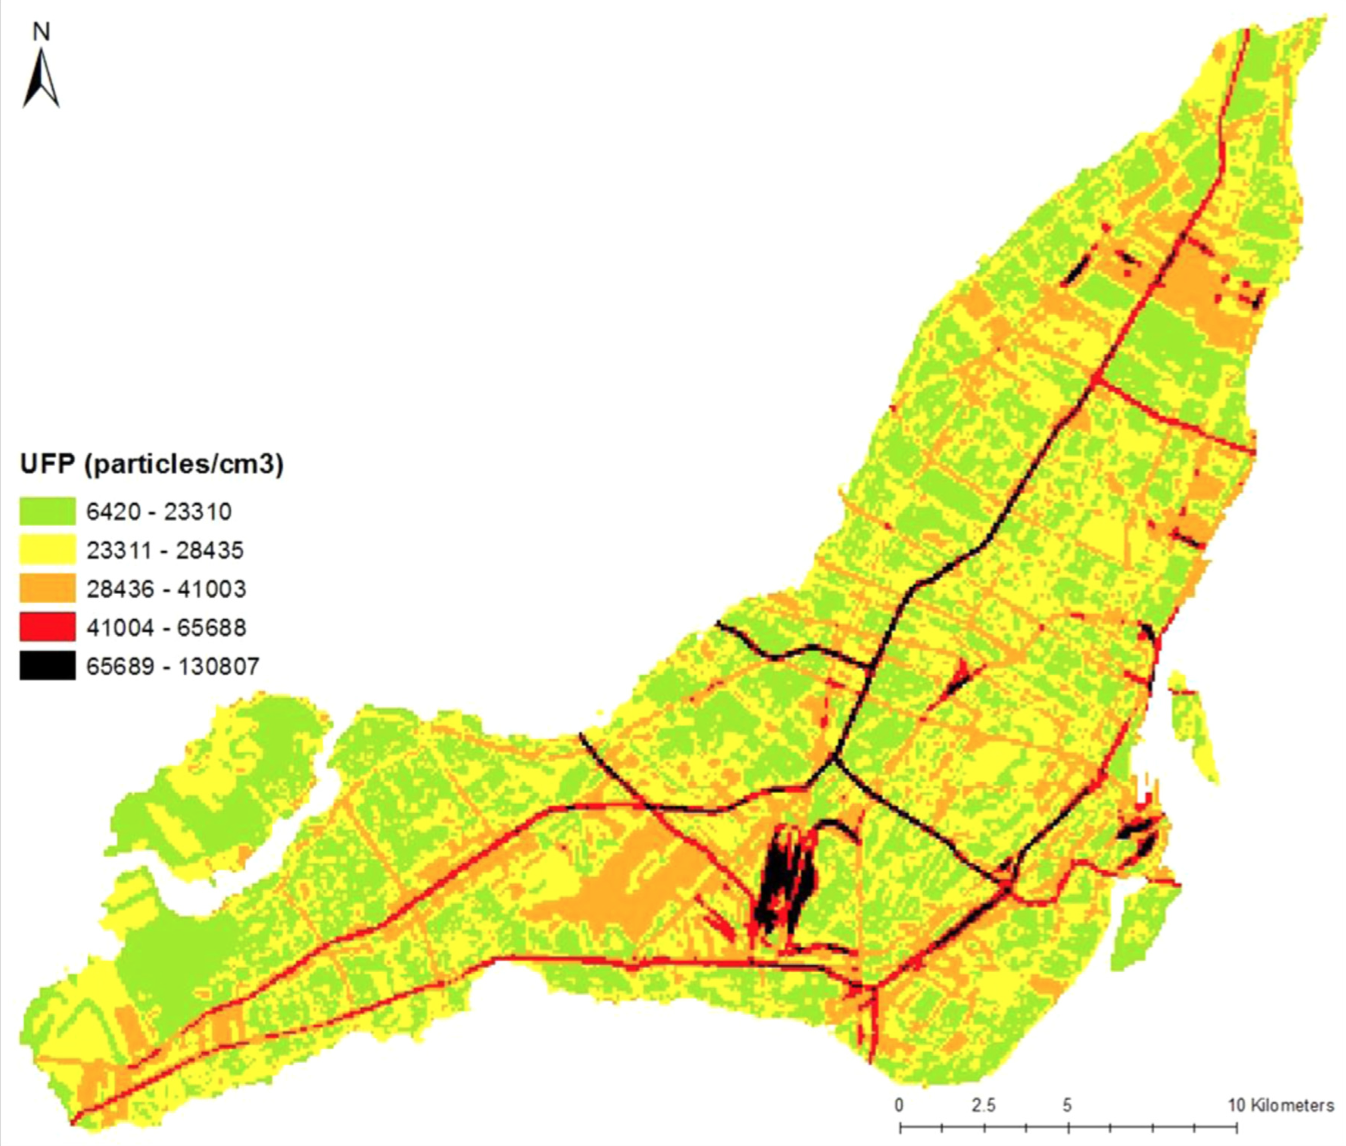
\includegraphics[height=5cm]{images/pollution_montreal.png}
\end{center}
\end{itemize}
précision $\sim$ 79\%.
\end{frame}

\begin{frame}
\frametitle{Plus proche voisins}

\begin{center}
\begin{tabular}{|c|c|c|}
  \hline
  score & methode & K \\
  \hline
  597.379 &  par polluant & K = 5\\
  \hline
  617.229 & par polluant & K = 3\\
  \hline
  613.892 & par polluant  & K = 4\\
  \hline
  613.892 & par polluant et par zone & K = 4\\
  \hline
\end{tabular}
\end{center}
\end{frame}

\begin{frame}
\frametitle{Méthode triviales}
\begin{itemize}
  \item
    valeur 0 : score $\sim$ 800
  \item
    moyenne globale : score $\sim$ 350
  \item regression linéraire sur les données dynamiques : score $\sim$ 450
\end{itemize}
\end{frame}

\begin{frame}
\frametitle{Gradient boosting}


Nous avons choisi de tester également un algorithme plus élaboré et plus adapté au problème. Nous avons choisi la random forest (ou communement appelée gradient boosting dans sa version boostée, pour améliorer les performances et réduire l'overfitting). En effet, les types de données du problème sont très diverses (mesure physiques, boolean, probabilités, ...), et bien qu'étant une régression, ce problème à une valeur décisionnelle importante. Comme nous l'avons vu, de nombreux paramètres interviennent de façon binaires. Par exemple beaucoup de vent ou beaucoup de pluie va entrainer automatiquement peu de polluant. Enfin, comme expliqué, le risque d'overfitting est énorme.

Nous avons donc fait tourner un algorithme de gradient boosting sur les données, après avoir interpolé les valeurs statiques manquantes, et avoir numéroté les différents polluants.

Dans notre protocole, pour se rendre d'un éventuel overfitting, nous avons séparé les données d'entrainement en train/validation par station. Ainsi nous sommes a priori exactement dans les mêmes conditions que lors de la prédiction des données test. En outre, les données test ayant exactement les mêmes paramètres dynamiques par zone que les données d'entrainement, il est impossible de faire de l'overfitting vis-à-vis de ces-derniers.

Nous avons comme résultat : 261 sur les données de validation, 302 sur les données test.

Sur les données de validation, nous avons des prédictions nettement meilleurs sur les microparticules (environ 100) que sur le $NO_2$ (465), ce qui rejoint notre analyse a priori des données. En outre, nous pouvons afficher l'importance relative des données lors de l'apprentissage.

\begin{center}
	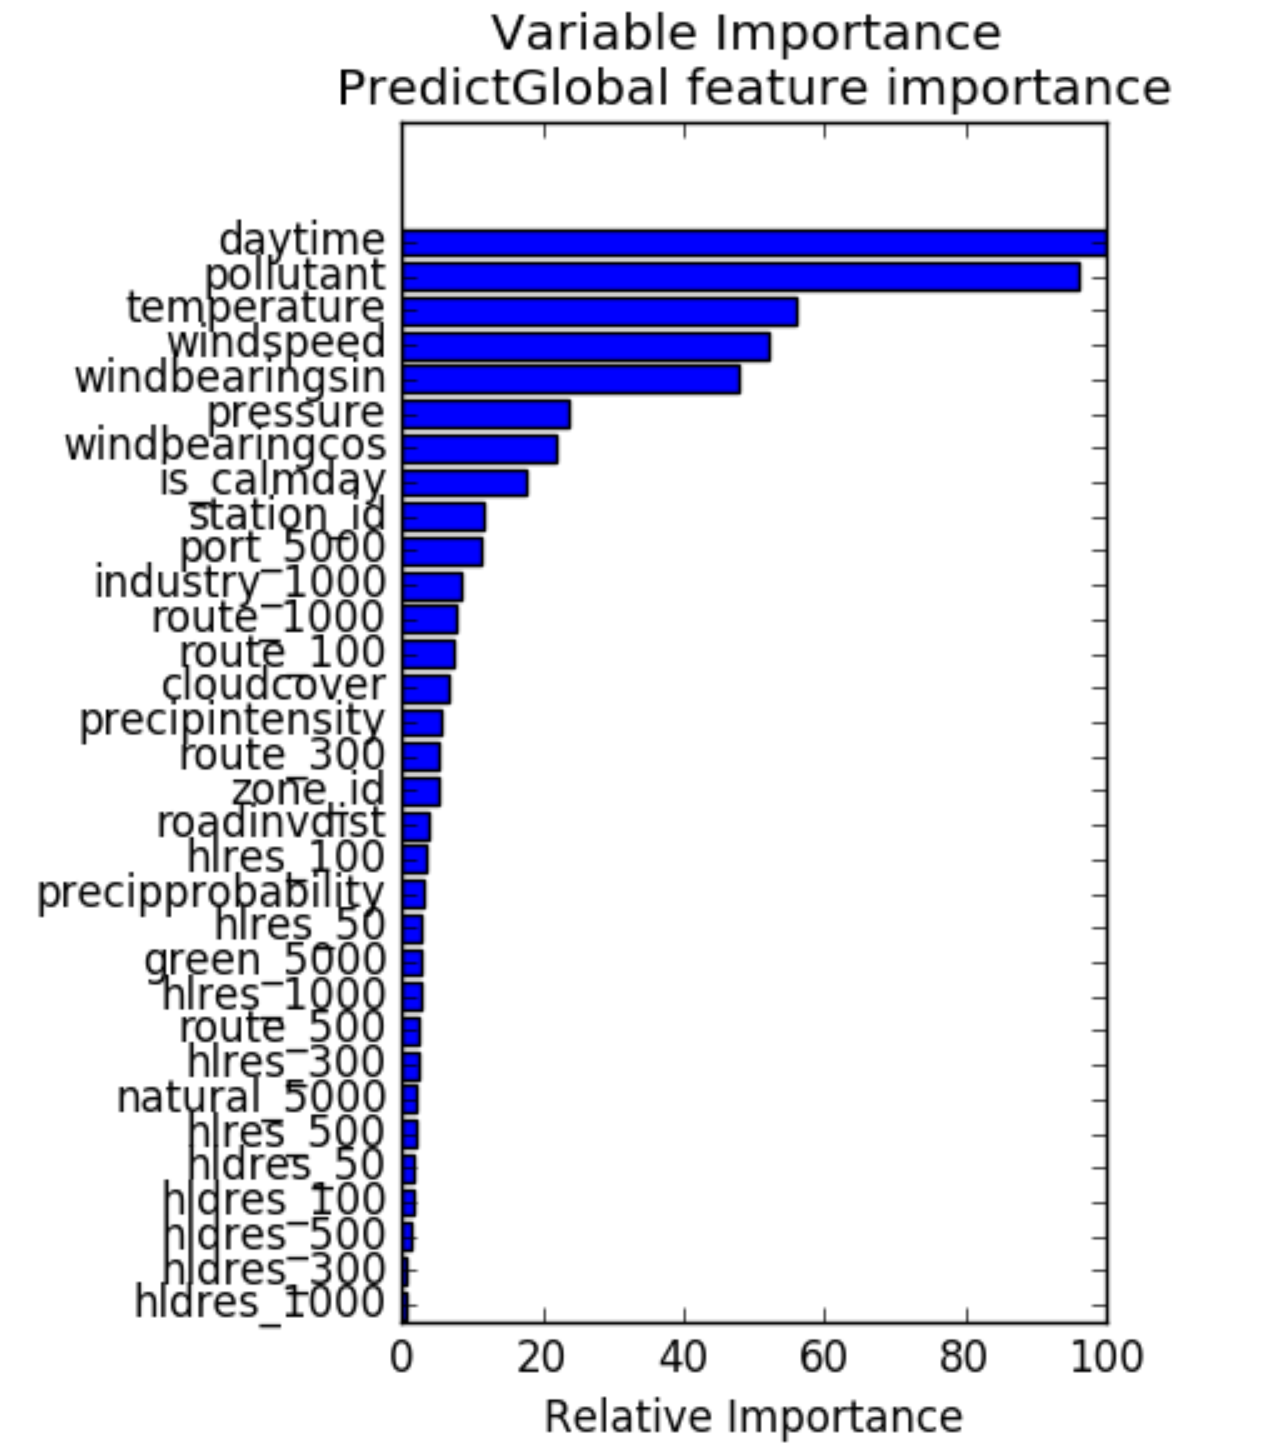
\includegraphics{images/importance feature global.png}
\end{center}

Ce graphique est très instructif, et on voit qu'il confirme nos raisonnements a priori sur les données. 
\begin{itemize}
	\item Le type de polluant a joué un rôle crucial dans la prédiction, ce qui nous confirme dans l'idée de séparer les polluants.
	\item Les données statiques ont rôle moindre par rapport aux données dynamique, ce qui est étonnant, surtout pour les routes qui devrait beaucoup influer sur le $NO_2$. Cela nous conforte dans l'idée que les paramètres statiques en notre possession sont peu pertinents.
	\item Le temps joue en rôle crucial également dans la prédiction. Bien que n'intervenant pas physiquement sur les polluant, il régit les activités humaines (et influe certain paramètres physiques), et donc la création de polluants.
	\item le numero de la station (stationid) joue en rôle important aussi, supérieur aux données statiques. %A commenter
\end{itemize}

\end{frame}


\begin{frame}

Comme prévu, l'algorithme de gradient boosting fonctionne mieux que la régression linéaire, et ses résultats nous encouragent encore plus à séparer les polluants. Nous avons donc appliqué l'algorithme précédent à chaque polluant indépendamment. 

En outre, étant donné l'importance du temps, qui est brut sous sa forme présente, nous avons divisé ce paramètre en plusieurs hyper-paramètres pertinents a priori : heure/mois/semaine/jour. Ainsi, nous utilisons un maximum les informations a priori sur l'influence des paramètres. Il pourrait aussi sembler utile de diviser également les données par zone, mais nous n'aurions alors plus assez de données statiques différentes pour apprendre (seulement 3).  

Les résultats obtenus sont bien meilleurs : 160 sur les données de validation, et 250 sur les données test. Nous n'avons pas optimisé cette méthode, usant de cross-validation ou autre technique d'ingenieure pour améliorer cette performance, car comme le prouve notre analyse et le benchmark, cela ne nous permettrait pas d'améliorer beaucoup notre score (passer de $15.5^2$ à $14^2$...).

\begin{center}
	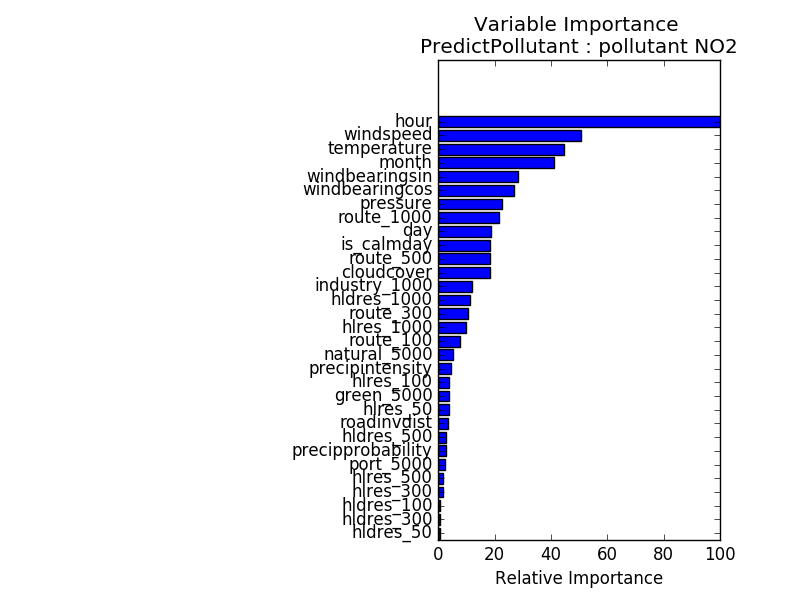
\includegraphics[width=0.3\linewidth]{images/NO2.png}
	%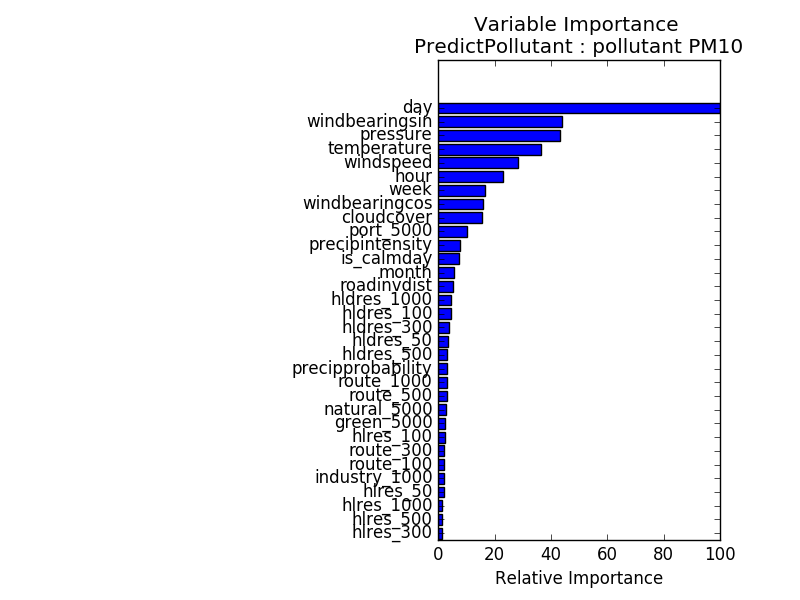
\includegraphics[width=0.3\linewidth]{images/PM10.png}
	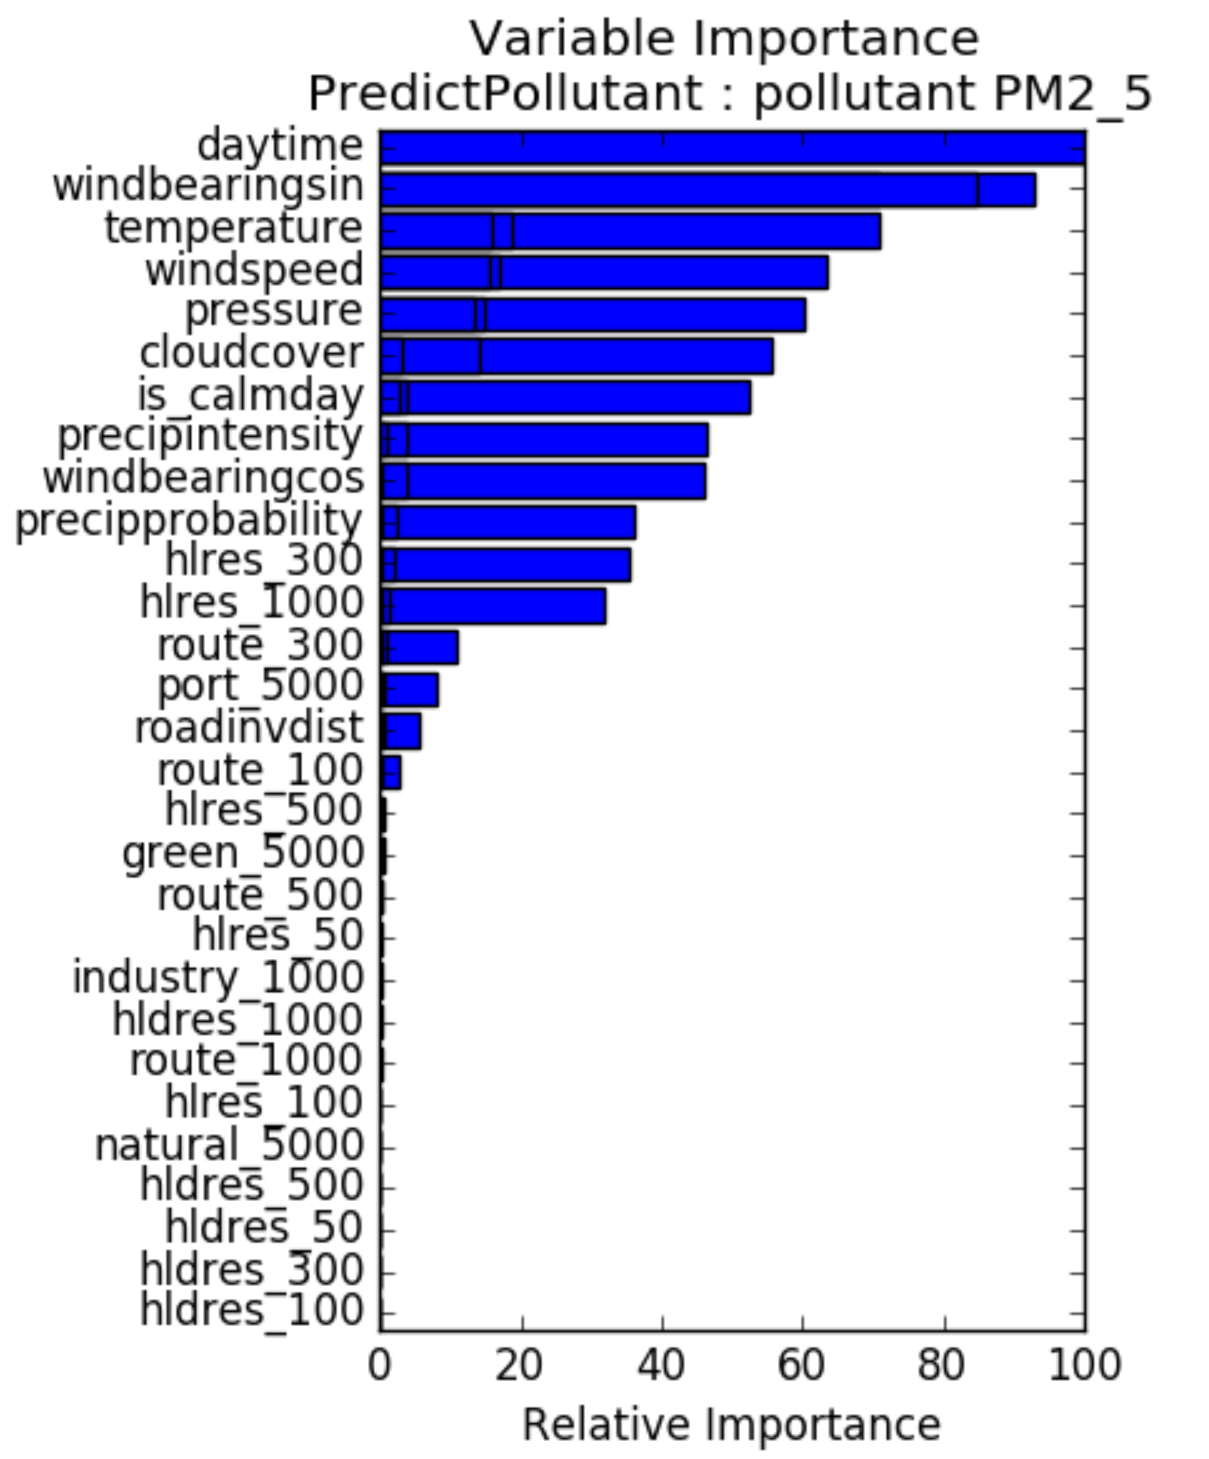
\includegraphics[width=0.3\linewidth]{images/PM25.png}
\end{center}

Les importances des paramètres ne font que confirmer ...
\end{frame}

\begin{frame}

Jusqu'ici nous n'avons pas encore essayé de palier à la bivalence des données d'entrainement. Les données dynamiques joue le rôle principal, mais le problème consiste à apprendre l'influence des données statiques (nous devons predire sur de nouvelles stations, et non sur de nouvelles données météorologiques). Dans l'application des algorithmes jusqu'à présent, les très maigres données statiques sont noyées dans la multitude des données dynamiques. Or le problème voudrait que l'on apprenne juste la dépendance envers les données dynamiques via les données statiques.

De plus, en première approximation, les données statiques et dynamiques jouent des rôles opposés. Les données statiques, purement liées aux activités humaines, régissent la création de polluant, alors que les données météorologiques régissent la dispersion des polluants. Nous pouvons donc modéliser la dépendance des paramètres, en notant $s$ pour statique, $d$ pour dynamique et $t$ pour le temps : $$ p(s,d) = g(s) - f(d)$$ avec g et f deux fonctions à apprendre. Cela nous permet de séparer les données et ainsi d'apprendre mieux la dépendance statique. Cependant, la séparation n'étant plus vraiment statique/dynamique, mais plutôt création/destruction de polluant. On inclut donc dans $s$, en plus des données statiques, les heures et le champ $is_calmday$.

En pratique, n'ayant pas accès à $f$ et $g$, nous apprenons les deux l'un après l'autre. On initialise $g$ par le maximum de polluant observé par station sur la durée donnée. Puis on apprend $f$, qu'on utilise pour apprendre $g$ et ainsi de suite, en espérant une convergence. 

% \begin{algorithm}[]
%   \KwData{Données d'entrainement strain, dtrain, ytrain}
%   \KwResult{fonctions f et g}
%   Initialiser $gtrain$ par $gtrain(strain) = \max_{dtrain}(Data(strain,dtrain))$ \;
%   \For{$i = 1$ to $iterationNumber $}{
%     $ftrain \leftarrow gtrain-ytrain$\;
%     Apprendre $f$ avec $f(dtrain) = ftrain$\;
%     $gtrain \leftarrow f(dtrain) + ytrain$\;
%     Apprendre $g$ avec $g(strain) = gtrain$\; 
%     $gtrain \leftarrow g(strain) $\;
%   }
%   \caption{Algorithme d'entrainement de la méthode séparation}
% \end{algorithm}

En pratique l'algorithme converge rapidement, et les résultats sont très convaincants. Nous obtenons sur les données de validation de meilleurs résultats qu'avec le gradient boosting. On obtient une erreur de 140 au lieu de 160, et l'erreur sur les données d'entrainements sont de  contre , ce qui laisse présager moins d'overfitting. Sur les données test, on obtient un score de , ce qui n'est pas très ettonnant compte tenu des remarques précédentes, on ne pouvait pas forcement faire beaucoup mieux, mais il nous semblait interessant d'essayer cette heuristique.
\end{frame}

\begin{frame}
  \bibliography{biblio.bib}
\end{frame}

\end{document}
